% vim: spl=pt
\begin{exercício}{Difração de Fresnel para abertura semi-plana}{ex6}
    Uma onda plana monocromática \(\psi_0 e^{ikz}\) incide normalmente sobre uma superfície opaca que ocupa todo o semi-plano \((x', y' < 0),\) como na figura abaixo. A luz é projetada numa tela a uma distância \(D\) da superfície. A intensidade da luz na tela obedece um padrão de difração \(I(y),\) sendo \(y\) a direção perpendicular à \(z\) paralela ao plano da figura.
    \begin{center}
        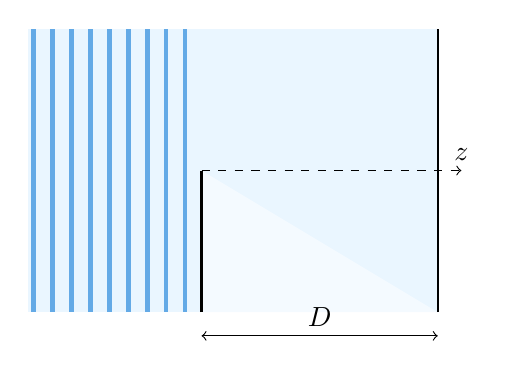
\begin{tikzpicture}[scale=0.6]

% Colors
\definecolor{lightblue}{RGB}{220,240,255}
\definecolor{Apertureblue}{RGB}{100,170,230}

% Parameters
\def\zAperture{0}
\def\zScreen{5}
\def\ApertureHeight{6}
\def\n{8}
\def\barWidth{0.1}
\def\spacing{0.3}
\def\height{6}

% Blue shaded region on the right
\fill[lightblue!60] ({\zAperture - (\n + 1.2)*(\barWidth + \spacing)},0) rectangle (\zScreen, \ApertureHeight);

% Background light cone
\fill[lightblue!30] 
    (\zAperture,0) -- (\zAperture, \height/2) -- (\zScreen, 0) -- cycle;

% Frentes de onda
\foreach \i in {0,...,\n} {
  \pgfmathsetmacro\x{\zAperture - (\i + 1)*(\barWidth+\spacing)}
  \fill[Apertureblue] (\x,0) rectangle ++(\barWidth,\ApertureHeight);
}

% Screen
\draw[thick] (\zScreen,0) -- (\zScreen,\ApertureHeight);

% 
\draw[dashed, ->] (\zAperture, \height/2) -- (1.1*\zScreen, \height/2) node[above] {\(z\)};

% Aperture edge
\draw[very thick] (\zAperture,0) -- (\zAperture,\ApertureHeight/2);

% Distance D
\draw[<->] (\zAperture, -0.5) -- (\zScreen, -0.5) node[above,midway] {\(D\)};
% \node[above] at ({0.5*(\zAperture+\zScreen)}, -0.5) {$D$};
\end{tikzpicture}
    \end{center}
    Obtenha a função \(I(y)\) em termos das integrais de Fresnel,
    \begin{equation*}
        F(\xi) = \int_0^\xi \dli{\zeta} \exp\left(i\frac{\pi}{2} \zeta^2\right) = C(\xi) + i S(\xi).
    \end{equation*}
    Sabendo que \(F(\xi) = - F(-\xi)\), que \(F(0) = 0,\) e que \(F(\xi) \to \frac{1 + i}{2}\) conforme \(\xi \to \infty\), estude o comportamento de \(I(y)\) para \(y \to \pm \infty\) e \(y = 0\). Expresse suas respostas em termos de \(I_0 = \abs{\psi_0}^2.\)
\end{exercício}
\begin{proof}[Resolução]
    
\end{proof}
